\documentclass[11pt]{report}
% PACKAGES
  \usepackage[a4paper,left=28mm,right=28mm,top=30mm,bottom=30mm]{geometry}
  \usepackage{graphicx,epstopdf}      % Used to import external graphics (figures)
  \usepackage{hyperref}       % Used for referring to links inside and outside the document
  \usepackage[table]{xcolor}  % To include colors 
  \usepackage{amsmath}        % For most of the math symbols and environments (such as \begin{align})
  \usepackage{amssymb}        % For using symbols in the document
  \usepackage{float}          % Arranging of figures on the page
  \usepackage[bf]{caption}    % Arranging the captions in floating environments [bf] makes the Figures bold
  \usepackage{subcaption}     % To arrange captions of subfigures
  \usepackage{booktabs}       % For standard tabular tables, with rules
  \usepackage{tabularx}       % For clean tables such as in the Nomenclature
  \usepackage{fancyhdr}       % Fancy headers
  \usepackage[colorinlistoftodos]{todonotes}      % To create todo notes
  \usepackage[nottoc,notlot,notlof]{tocbibind}    % Add bibliography to content
  \usepackage{bm}             % Make bold symbols
  \usepackage{lipsum}
  \usepackage{parskip}
% LAY-OUT
  % \usepackage{pdfpages}

  % \usepackage{pdflscape}

   \renewcommand\thesection{\arabic{section}}

  % \usepackage[mathletters]{ucs}
  % \usepackage[utf8x]{inputenc}
  %Bibliography for references, with reference style options
  \usepackage[
  backend=biber,
  bibstyle=ieee,
  citestyle=numeric-comp,
  dashed=false,
  url = false,
  maxnames=8,
  maxcitenames=2,
  mincitenames=1,
  sorting=none,
  isbn = false,
  doi = false
  ]{biblatex}
  \addbibresource{references.bib}

  %Set the page style
  \pagestyle{fancy}
  \fancyhead[L]{\ifodd\value{page} \slshape\nouppercase{\rightmark} \else \fi}
  \fancyhead[R]{\ifodd\value{page} \else \slshape\nouppercase{\leftmark} \fi}
  \chead{ }
  \lfoot{}
  \rfoot{}
  \cfoot{\small\thepage}


  %Give colors to links/refs etc
  \hypersetup{colorlinks, linkcolor={blue!0!black}, 
                          citecolor={blue!70!black}, 
                           urlcolor={blue!80!}} 
                       
  %% Set up numbering and spacing
  \numberwithin{equation}{section}        %Number the equations per section
  \numberwithin{figure}{section}          %Number the figures per section
  \numberwithin{table}{section}           %Number the tables per section
  \captionsetup[table]{skip=1pt}          %Skip 1 pt after a table
  \captionsetup[figure]{skip=3.5pt}       %Skip 4 pt after a figure
  \setcounter{secnumdepth}{3}             %Count up to the subsubsection 
  \setcounter{topnumber}{1}               %Number of floats at top of a page (default is 2)

  %%%%% proof/theorem/definition boxes

  \usepackage{cleveref}
  \usepackage[most]{tcolorbox}
  \newtcbtheorem{Theorem}{Theorem}{
    enhanced,
    sharp corners,
    attach boxed title to top left={
      yshifttext=-1mm
    },
    colback=white,
    colframe=blue!75!black,
    fonttitle=\bfseries,
    boxed title style={
      sharp corners,
      size=small,
      colback=blue!75!black,
      colframe=blue!75!black,
    } 
  }{thm}

  \newtcbtheorem{Definition}{Definition}{
    enhanced,
    sharp corners,
    attach boxed title to top left={
      yshifttext=-1mm
    },
    colback=white,
    colframe=blue!25,
    fonttitle=\bfseries,
    coltitle=black,
    boxed title style={
      sharp corners,
      size=small,
      colback=blue!25,
      colframe=blue!25,
    } 
  }{def}

  \newtcbtheorem[no counter]{Proof}{Proof}{
    enhanced,
    sharp corners,
    attach boxed title to top left={
      yshifttext=-1mm
    },
    colback=white,
    colframe=blue!25,
    fonttitle=\bfseries,
    coltitle=black,
    boxed title style={
      sharp corners,
      size=small,
      colback=blue!25,
      colframe=blue!25,
    } 
  }{prf}
% DEFINITIONS
  %% Titlepage definitions
  \newcommand{\deltitle}{Impact-Aware Control for a Dual-Arm Setup}      %Your project title
  \newcommand{\StudentName}{Gijs van den Brandt}  %Student name
  \newcommand{\StudentID}{1257110}                    %Your student number
  % \newcommand{\DCcode}{2021.109}                      %Get your DC code from the D&C secretariat

  %% Operators
  \DeclareMathOperator\sign{sgn}                      %Sign function
  \DeclareMathOperator\diag{diag}                     %Diagonal operator
  \DeclareMathOperator\imag{Imag}                     %Imaginary part of complex variable
  \DeclareMathOperator\real{Real}                     %Real part of complex variable
  \DeclareMathOperator*{\argmin}{\arg\!\min}          %Argmin operator
  \newcommand{\norm}[1]{\left\lVert#1\right\rVert}    %Norm operator

  %% Variable definition
  \newcommand{\R}{\mathbb{R}}                         % Set of real numbers
  \newcommand{\C}{\mathbb{C}}                         % Set of complex numbers

\begin{document}

% Summary 
  \section*{Progress meeting 10 | 24 October, 2022}


  \section*{1. Progress}
  \begin{itemize}
  \item \textbf{Teleoperation:} Last time, I mentioned that the velocity reference results in more responsive tracking of the VR device. This was paired with the safety limits of the robot being exceeded in edge cases. It was suggested that I look into the task weights, however in section xxx I show that changing weights is not a solution. Instead of altering weights, I solved the problem by tuning the reference augmentation.
    
  \item \textbf{Impact detection:} I implemented impact detection using a jump-aware filter, a prediction function, and a bounding function as described by Mark Rijnen. In section xxx, I argue that a small moving window for the filter is better than a large window. As a result, the prediction is equivalent to a linear extrapolation and the jump-aware filter is redundant. This is supported by experimental data.

  Furthermore, impact detection based on the estimated force rate was compared to Mark Rijnen's approach with position measurements. Comparatively, the force rate method has a lower response time as was already suggested by Sven.

  \item \textbf{Learning from demonstration:} An experiment was performed where the robot stamps on the table. This is further explained in section xxx. Impedance control without reference spreading was compared to impedance control with reference spreading in vertical direction. The addition of reference spreading reduced the required control effort and joint torques at the time of impact. The implementation should be expanded to also support reference spreading in rotational DoF's so that more complex tasks than just stamping can be performed. Furthermore, an intermediate impact control mode should be investigated.

  \item \textbf{Use case:} 
  \end{itemize}

  \section*{2. Agenda}
  During the meeting, I would like to discuss the following points:

  \begin{itemize}
      \item  
      \item 
  \end{itemize}

  \section*{3. Next steps}

  \begin{itemize}
      \item  
      \item 
  \end{itemize}

  \section*{4. Long-term planning}
  Below is the current long-term planning for the project phase. The description of the labeled subjects are given in the preparation phase report and are also provided on the next page.

  \begin{figure}[H]
  \centering
  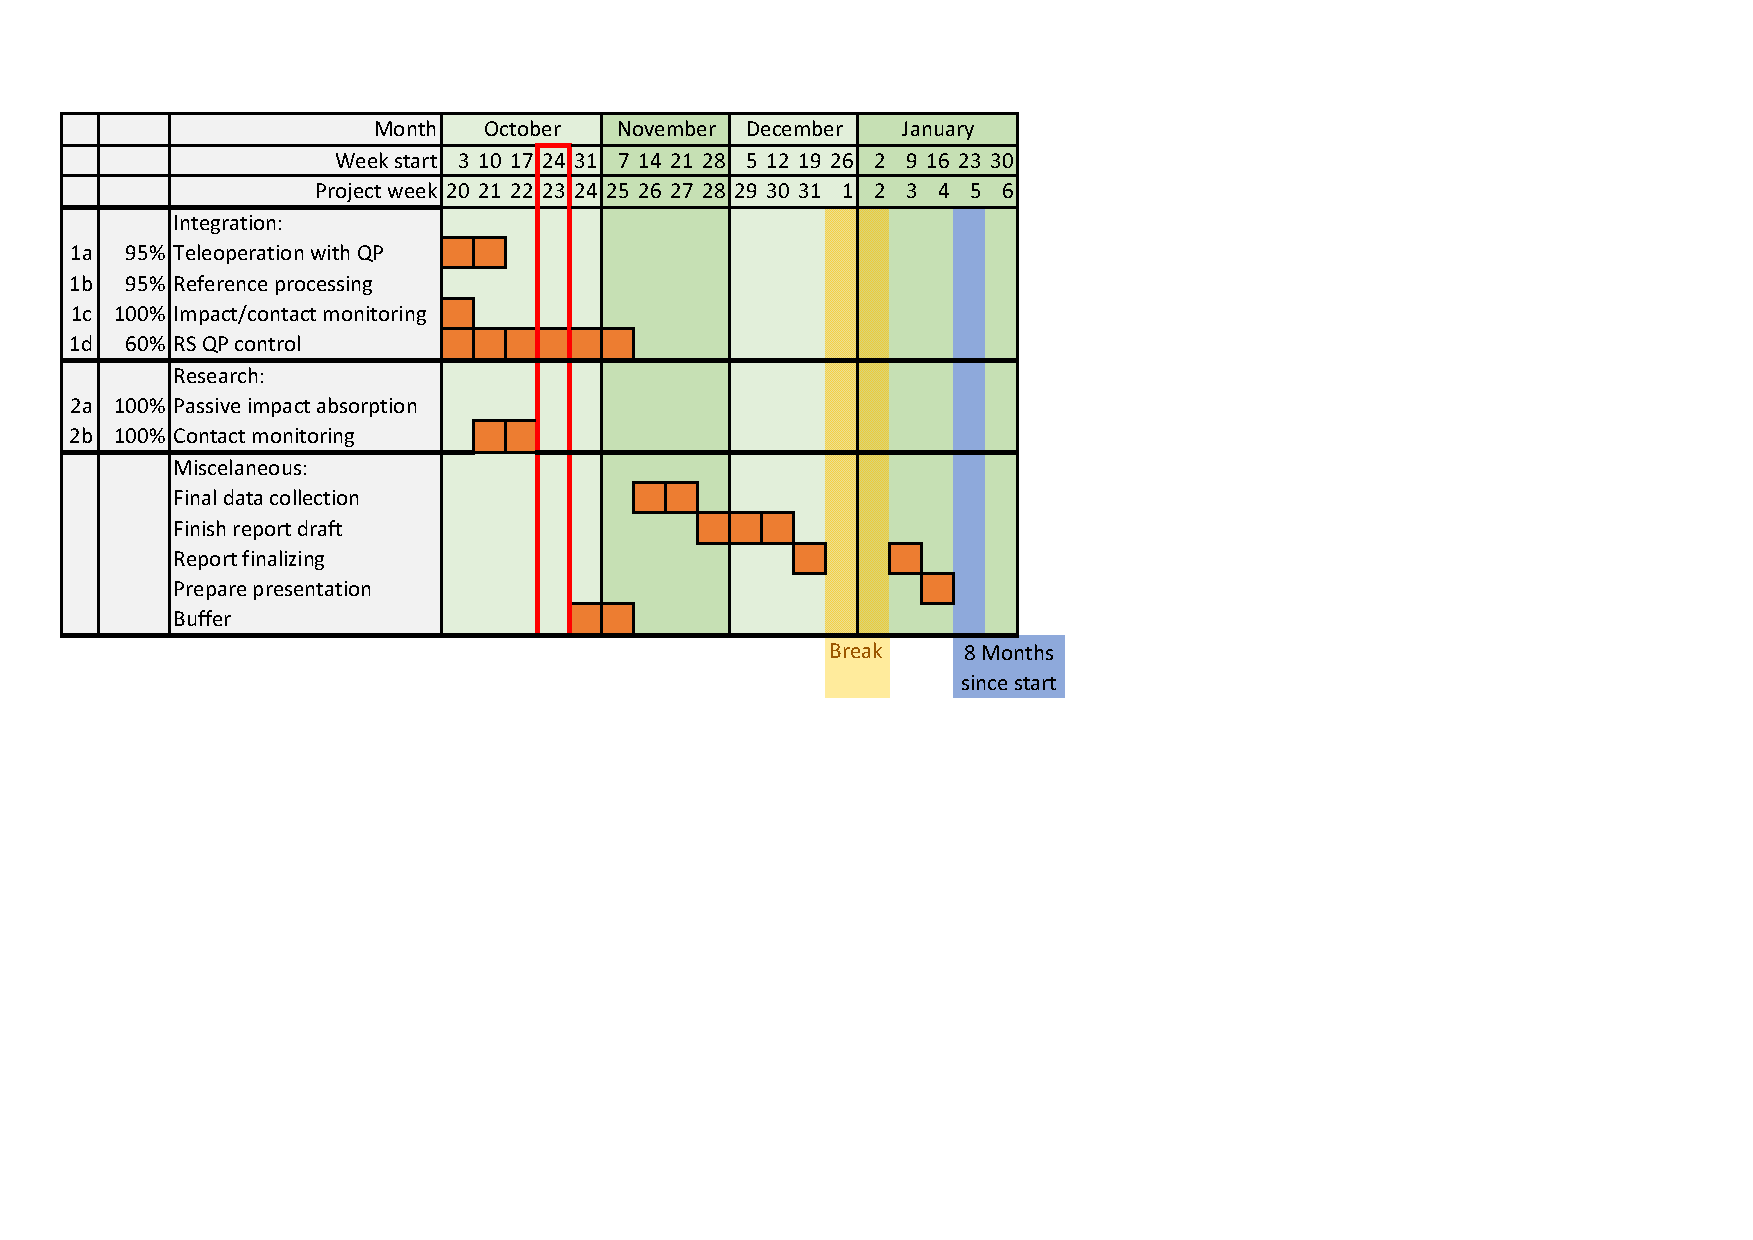
\includegraphics[width=0.7\textwidth, trim={0.87cm 9.5cm 10cm 1.5cm},clip]{Graphics/planning v2.pdf}

  \label{fig:my_label}
  \end{figure}

  \begin{enumerate}
  \item[1a] \textbf{Translating dual-arm teleoperation to the physical setup.} The existing implementation in simulation already uses the mc\_rtc interface, meaning that the switch to reality shouldn't pose an issue. Nevertheless, this step also involves getting familiar with the software, which increases the anticipated time for this step.
  \item[1b] \textbf{Extracting references from the demonstration data.} The demonstrated trajectories should be split into ante-impact and post-impact sections, and extended to facilitate RS. Furthermore multiple measurements should be used to fit ProMPs, after which a reference can be generated. It is also key to identify which data should be learned from the demonstration. This is not limited to choosing between a force or position reference, but can also consists of learning properties of the environment, e.g. friction cones or box inertia, that are crucial to a dual-arm box grabbing scenario.
  \item[1c] \textbf{Integrating impact detection and contact monitoring in mc\_rtc.} The majority of the impact detector's complexity resides in the momentum observer; however, Franka Emika's software already has an integrated momentum observer. This still leaves tuning of the impact detecting algorithms which might be time consuming. Furthermore an analysis comparing the available methods could be worthwhile. Factors which determines the effectivity of the impact detection algorithm include speed of detection, as well as reliability, i.e. the rate of false positives. The addition of objects that cause unexpected impacts is not considered a part of the research scope.
  \item[1d] \textbf{Configuring QP controllers for the ante-impact, intermediate, and post-impact phase.} For each of the phases, it is important to address the redundancy in the arms' degrees of freedom. After that, control for the ante-impact phase should be trivial. For the intermediate phase, it is expected that ante-impact reference tracking without velocity feedback should be applicable on a dual-arm robot, though this might prove to be false, in which case other methods should be investigated. During post-impact control, the challenge will be maintaining non-slip contact with the box. It is difficult to say how well the results from simulations can be repeated with torque control, where the state of the box can not be sensed to be used in the QP controller.
   \item[2a] \textbf{Passive impact absorption:} A soft cover for the end effector will be designed. Such a cover can be connected to the Panda by connecting bolts to the so-called flange interface. A mold will be created using 3D printing to allow for casting of various silicone soft covers. Design parameters -- i.e. material properties (controlled by choosing different kinds of silicone) and soft cover thickness -- will be analyzed experimentally. A systematic comparison between various designs will require an experiment plan including a realistic testing scenario. Evaluation of performance can be based on the oscillatory response in position and force after establishing contact. Furthermore multiple scenarios with various box surface properties and robot poses should be considered.
  
  \item[2b] \textbf{Contact monitoring:} When investigating contact monitoring, two approaches can be taken: either using proprioceptive or exteroceptive sensors. A possible improvement for contact monitoring using proprioceptive sensors could be to wait a fixed time starting from the last detected impact, rather than waiting a fixed time from the first impact. As for exteroceptive sensors, they can be a hurdle for large-scale commercial applications as they are not integrated in the robot. However, if a soft cover is to be mounted to the end effector, including tactile sensors for impact and contact monitoring becomes more feasible. Practical questions such as which tactile sensor to use and how to integrate it could be addressed, though this is not absolutely necessary for completing the research goals, and therefore has a low priority.
  \end{enumerate}
% main text
  \newpage
  \section{First subject}

  \section{Second subject}
% BIBLIOGRAPHY

  \newpage
  \addcontentsline{toc}{chapter}{References}
  \printbibliography[title=References]

  \newpage
  \thispagestyle{empty} \ \newpage


\end{document}